% !TEX program = xelatex
% !BIB program = biber
%==============================================================================
% LAPORAN AKHIR PROYEK PENGGANTI UAS
% Mata Kuliah Kecerdasan Buatan | Teknik Komputer - Universitas Indonesia
% Semester Genap 2025/2026 | Kelompok 06
%
% Kompilasi:
%   xelatex laporan-akhir-kel06.tex
%   biber   laporan-akhir-kel06
%   xelatex laporan-akhir-kel06.tex
%   xelatex laporan-akhir-kel06.tex
%
% Gambar diambil dari ../results/figures/ (relatif terhadap folder submission/).
%==============================================================================

\documentclass[11pt,a4paper,oneside]{report}

%------ Bahasa & Font --------------------------------------------------------
\usepackage{fontspec}
\setmainfont{Times New Roman}
\setmonofont{Consolas}[Scale=0.92]

%------ Geometri & Spasi -----------------------------------------------------
\usepackage[a4paper,margin=2.5cm]{geometry}
\usepackage{setspace}
\onehalfspacing
\setlength{\parskip}{0.5em}

%------ Paket Pendukung ------------------------------------------------------
\usepackage{graphicx}
\graphicspath{{../results/figures/}{./}}
\usepackage{amsmath,amssymb,amsfonts}
\usepackage{booktabs}
\usepackage{array}
\usepackage{tabularx}
\usepackage{longtable}
\usepackage{enumitem}
\usepackage{xcolor}
\usepackage{listings}
\usepackage{hyperref}
\usepackage{titlesec}
\usepackage{tcolorbox}
\usetikzlibrary{shapes.geometric, arrows.meta, positioning, calc}
\usepackage{float}
\usepackage{caption}
\usepackage{subcaption}
\usepackage[backend=biber,style=ieee]{biblatex}

%------ Penyesuaian Bahasa Indonesia -----------------------------------------
\renewcommand{\chaptername}{BAB}
\renewcommand{\contentsname}{DAFTAR ISI}
\renewcommand{\listfigurename}{DAFTAR GAMBAR}
\renewcommand{\listtablename}{DAFTAR TABEL}
\renewcommand{\bibname}{DAFTAR PUSTAKA}
\renewcommand{\appendixname}{LAMPIRAN}
\renewcommand{\figurename}{Gambar}
\renewcommand{\tablename}{Tabel}

%------ Format Bab -----------------------------------------------------------
\titleformat{\chapter}[display]
  {\normalfont\Large\bfseries\centering}
  {\chaptername\ \thechapter}{12pt}{\Large}
\titlespacing*{\chapter}{0pt}{-20pt}{20pt}

%------ Hyperref -------------------------------------------------------------
\hypersetup{
  colorlinks=true,
  linkcolor=black,
  urlcolor=blue,
  citecolor=black,
  breaklinks=true,
  pdftitle={Laporan Akhir - Klasifikasi DDoS LSTM/GRU/RF - Kelompok 06},
  pdfauthor={Kelompok 06}
}

%------ Listing untuk JSON ---------------------------------------------------
\lstdefinelanguage{json}{
  basicstyle=\ttfamily\footnotesize,
  showstringspaces=false,
  breaklines=true,
  frame=single,
  rulecolor=\color{gray!50},
  string=[s]{"}{"},
  stringstyle=\color{blue!60!black}
}

%------ Bibliography ---------------------------------------------------------
\addbibresource{referensi.bib}

%==============================================================================
\begin{document}

%==============================================================================
% HALAMAN SAMPUL
%==============================================================================
\begin{titlepage}
\centering
\vspace*{1cm}

{\Large\bfseries LAPORAN AKHIR \par}
{\large PROYEK PENGGANTI UAS \par}
\vspace{0.3cm}
{\large Mata Kuliah Kecerdasan Buatan \par}
{\large Semester Genap 2025/2026 \par}

\vspace{1.5cm}

{\LARGE\bfseries Klasifikasi Lalu Lintas Jaringan DDoS Menggunakan LSTM, GRU, dan Random Forest pada Dataset CIC-DDoS2019 \par}
\vspace{0.5cm}
{\large Perbandingan Arsitektur Temporal Deep Learning dan Machine Learning Tradisional untuk Deteksi Serangan Jaringan \par}

\vspace{2cm}

{\large Disusun oleh: \par}
\vspace{0.5cm}
\begin{tabular}{rl}
Calvin Wirathama Katoroy & NPM. 2306242395 \\
Syahmi Hamdani           & NPM. 2306220532 \\
Christover Angelo        & NPM. 2306220323 \\
Matthew Immanuel         & NPM. 2306221024 \\
\end{tabular}

\vspace{1.5cm}

{\large Dosen Pengampu: \par}
{\large Muhammad Firdaus Syawaludin Lubis, Ph.D. \par}

\vfill

{\large DEPARTEMEN TEKNIK KOMPUTER \par}
{\large FAKULTAS TEKNIK \par}
{\large UNIVERSITAS INDONESIA \par}
{\large MEI 2026 \par}
\end{titlepage}

%==============================================================================
% LEMBAR PERNYATAAN ORISINALITAS
%==============================================================================
\chapter*{LEMBAR PERNYATAAN ORISINALITAS}
\addcontentsline{toc}{chapter}{Lembar Pernyataan Orisinalitas}

Kami yang bertandatangan di bawah ini menyatakan bahwa laporan ini beserta seluruh isinya (termasuk Sub-bab IV.x masing-masing anggota dan berkas \texttt{metadata.json} yang merupakan bagian tidak terpisahkan) adalah hasil karya kelompok kami sendiri. Setiap kutipan, kode, atau gambar yang berasal dari sumber lain telah disitasi dengan benar. Penggunaan AI \textit{assistant} telah dideklarasikan secara jujur pada Sub-bab IV.x.2.

\vspace{1.5cm}

\noindent
\begin{tabular}{p{0.45\textwidth}p{0.45\textwidth}}
\centering Calvin Wirathama Katoroy & \centering Syahmi Hamdani \tabularnewline
\centering NPM. 2306242395 & \centering NPM. 2306220532 \tabularnewline
\vspace{1.5cm} & \vspace{1.5cm} \tabularnewline
\centering (\hspace{4cm}) & \centering (\hspace{4cm}) \tabularnewline
\end{tabular}

\vspace{1cm}

\noindent
\begin{tabular}{p{0.45\textwidth}p{0.45\textwidth}}
\centering Christover Angelo & \centering Matthew Immanuel \tabularnewline
\centering NPM. 2306220323 & \centering NPM. 2306221024 \tabularnewline
\vspace{1.5cm} & \vspace{1.5cm} \tabularnewline
\centering (\hspace{4cm}) & \centering (\hspace{4cm}) \tabularnewline
\end{tabular}

%==============================================================================
% DAFTAR ISI, GAMBAR, TABEL
%==============================================================================
\tableofcontents
\listoffigures
\listoftables

%==============================================================================
% ABSTRAK
%==============================================================================
\chapter*{ABSTRAK}
\addcontentsline{toc}{chapter}{Abstrak}

Proyek ini membandingkan tiga arsitektur model untuk mengklasifikasikan lalu lintas jaringan secara biner (normal vs.\ serangan DDoS) pada dataset CIC-DDoS2019 versi \textit{cleaned} dari Kaggle (431.371 sampel, 17 jenis serangan). LSTM dipilih sebagai model utama karena kemampuannya menangkap dependensi temporal dalam urutan aliran jaringan; GRU dan Random Forest digunakan sebagai model baseline. Pipeline preprocessing mencakup seleksi 16 fitur CICFlowMeter, StandardScaler (fit pada \textit{train set} saja), stratified 70/15/15 split (seed 42), dan \textit{sliding window} seq\_len=10 untuk model sekuensial. Seluruh training dilakukan di Google Colab dengan GPU T4.

Hasil evaluasi pada \textit{test set}: LSTM mencapai F1-score 0,9976 (\textit{accuracy} 99,63\%, FPR 0,46\%, AUC 99,96\%); GRU mencapai F1-score 0,9975 (\textit{accuracy} 99,61\%, FPR 0,28\%, AUC 99,96\%); Random Forest mencapai F1-score 0,9992 (\textit{accuracy} 99,87\%, FPR 0,15\%, AUC 99,98\%). Random Forest mengungguli kedua model \textit{deep learning} pada semua metrik, mengindikasikan bahwa fitur CICFlowMeter yang sudah ter-\textit{engineer} secara informatif sudah cukup representatif untuk tugas ini tanpa pemodelan temporal tambahan. \textit{Hyperparameter tuning} terdokumentasi: 6 eksperimen LSTM, 6 eksperimen GRU, dan 6 eksperimen Random Forest.

\vspace{1em}
\noindent\textbf{Kata kunci:} LSTM, GRU, Random Forest, deteksi DDoS, klasifikasi lalu lintas jaringan

%==============================================================================
% BAB I - PENDAHULUAN & DEFINISI MASALAH
%==============================================================================
\chapter{PENDAHULUAN \& DEFINISI MASALAH}
\label{bab:pendahuluan}

\section{Topik yang Dipilih}

Topik yang dipilih adalah \textbf{RNN / GRU / LSTM} (Topik 2). Lalu lintas jaringan pada dasarnya bersifat sekuensial: sebuah aliran jaringan terdiri dari serangkaian paket yang memiliki ketergantungan temporal satu sama lain. LSTM, sebagai varian \textit{Recurrent Neural Network} (RNN) dengan mekanisme \textit{gating}, mampu menangkap pola temporal jangka panjang yang relevan dengan karakteristik serangan DDoS, seperti lonjakan volume paket yang terstruktur dalam waktu. Sebuah lonjakan pada $t=47$ hanya bernilai anomali dalam konteks rentang $t=44..46$; pendekatan non-sekuensial seperti Random Forest tidak dapat menangkap konteks ini secara langsung.

Pemilihan topik ini juga berkaitan dengan penelitian laboratorium di Network Laboratory DTE FT UI~\cite{breiman2001}, di mana Random Forest telah digunakan sebagai diskriminator dalam pipeline deteksi DDoS berbasis SIEM Wazuh. Proyek ini mengevaluasi apakah LSTM dan GRU dapat memberikan performa yang lebih baik dibandingkan Random Forest sebagai komponen klasifikasi dalam pipeline tersebut.

\section{Rumusan Masalah}

\begin{enumerate}[label=RM\arabic*.,leftmargin=*]
    \item Seberapa baik model LSTM mampu mengklasifikasikan lalu lintas jaringan sebagai normal atau serangan DDoS pada dataset CIC-DDoS2019, diukur dengan F1-score, \textit{accuracy}, FPR, dan AUC-ROC?
    \item Apakah model LSTM memberikan performa yang lebih baik dibandingkan GRU dan Random Forest pada dataset yang sama?
    \item Bagaimana pengaruh \textit{hyperparameter} utama (hidden\_size, seq\_len, num\_layers, dropout) terhadap performa LSTM dan GRU dalam konteks deteksi DDoS?
\end{enumerate}

\section{Tujuan Proyek}

\begin{enumerate}[label=T\arabic*.,leftmargin=*]
    \item Menerapkan dan melatih model LSTM untuk klasifikasi biner lalu lintas jaringan pada dataset CIC-DDoS2019 dengan evaluasi komprehensif pada metrik accuracy, F1-score, FPR, dan AUC-ROC.
    \item Membandingkan performa LSTM, GRU, dan Random Forest secara kuantitatif pada dataset dan metrik yang sama untuk menentukan arsitektur terbaik dalam konteks deteksi DDoS.
    \item Mendokumentasikan eksperimen \textit{hyperparameter tuning} secara sistematis (minimal 6 eksperimen per model) untuk menganalisis sensitivitas model terhadap perubahan konfigurasi.
    \item Menganalisis keterbatasan, potensi bias, dan implikasi etika penggunaan model pada lingkungan produksi nyata.
\end{enumerate}

\section{Ruang Lingkup \& Batasan}

Proyek ini \textbf{mencakup}: (1) klasifikasi biner lalu lintas jaringan (normal vs.\ DDoS) pada dataset CIC-DDoS2019; (2) perbandingan tiga arsitektur model menggunakan metrik yang seragam; (3) \textit{hyperparameter tuning} terdokumentasi dengan minimal 6 eksperimen per model; (4) analisis etika, bias, dan keterbatasan model untuk klaim bonus B3.

Proyek ini \textbf{tidak mencakup}: (1) klasifikasi multi-kelas per jenis serangan DDoS; (2) \textit{deployment} model ke sistem produksi atau integrasi langsung dengan Wazuh SIEM; (3) pengumpulan dataset mandiri (menggunakan dataset benchmark publik); (4) pengujian pada jenis serangan yang tidak ada dalam CIC-DDoS2019 (mis.\ QUIC-based DDoS, HTTP/2 RST flood); (5) \textit{online learning} atau adaptasi model terhadap distribusi traffic baru.

%==============================================================================
% BAB II - PENDEKATAN AI
%==============================================================================
\chapter{PENDEKATAN AI}
\label{bab:pendekatan}

\section{Tinjauan Pustaka (\textit{Related Work})}

\begin{table}[h!]
\centering
\caption{Ringkasan tinjauan pustaka}
\label{tab:related-work}
\begin{tabularx}{\textwidth}{p{3.2cm}p{2.8cm}p{2.2cm}p{2.5cm}p{2.5cm}}
\toprule
\textbf{Penulis (Th.)} & \textbf{Metode} & \textbf{Dataset} & \textbf{Hasil} & \textbf{Keterbatasan} \\
\midrule
Sharafaldin et al.\ (2019)~\cite{sharafaldin2019} & Rilis dataset CIC-DDoS2019 & CIC-DDoS2019 (UNB) & Benchmark dataset untuk 12 jenis serangan DDoS & Hanya lingkungan testbed; tidak mencerminkan ISP produksi \\
\addlinespace
Hochreiter \& Schmidhuber (1997)~\cite{hochreiter1997} & LSTM dengan \textit{gating mechanism} & Sintetis & Mengatasi \textit{vanishing gradient} pada sekuensi panjang & Komputasi lebih berat dibanding RNN standar \\
\addlinespace
Cho et al.\ (2014)~\cite{cho2014} & GRU sebagai penyederhanaan LSTM & Teks (NMT) & Performa setara LSTM dengan lebih sedikit parameter & Validasi terbatas pada domain NLP \\
\addlinespace
Breiman (2001)~\cite{breiman2001} & Random Forest (bagging ensemble) & UCI benchmark & Performa tinggi pada tabular data tanpa tuning intensif & Tidak dapat menangkap dependensi temporal antar sampel \\
\addlinespace
Roopak et al.\ (2019)~\cite{roopak2019} & LSTM, CNN, MLP pada IoT IDS & NSL-KDD & LSTM F1 0.998 untuk deteksi intrusi & Menggunakan NSL-KDD (dataset lama); tidak mencakup DDoS modern \\
\bottomrule
\end{tabularx}
\end{table}

Berbeda dari Roopak et al.~\cite{roopak2019} yang menggunakan dataset NSL-KDD dengan arsitektur tunggal, proyek ini mengevaluasi tiga arsitektur (LSTM, GRU, RF) secara komparatif pada CIC-DDoS2019, dataset yang lebih baru dan mencakup jenis serangan DDoS yang lebih beragam, dengan dokumentasi \textit{hyperparameter tuning} yang sistematis.

\section{Landasan Teori Model yang Dipilih}

\subsection*{LSTM (\textit{Long Short-Term Memory})}

LSTM~\cite{hochreiter1997} mengatasi masalah \textit{vanishing gradient} pada RNN standar melalui mekanisme tiga buah \textit{gate} dan sebuah \textit{cell state} $c_t$. Pada setiap \textit{timestep} $t$, diberikan input $x_t \in \mathbb{R}^{d}$ dan \textit{hidden state} sebelumnya $h_{t-1} \in \mathbb{R}^{h}$, LSTM menghitung:

\begin{align}
f_t &= \sigma\!\left(W_f [h_{t-1},\, x_t] + b_f\right) & &\text{(\textit{forget gate})} \label{eq:forget}\\
i_t &= \sigma\!\left(W_i [h_{t-1},\, x_t] + b_i\right) & &\text{(\textit{input gate})} \label{eq:input}\\
\tilde{c}_t &= \tanh\!\left(W_c [h_{t-1},\, x_t] + b_c\right) & &\text{(\textit{cell candidate})} \label{eq:candidate}\\
c_t &= f_t \odot c_{t-1} + i_t \odot \tilde{c}_t & &\text{(\textit{cell state update})} \label{eq:cell}\\
o_t &= \sigma\!\left(W_o [h_{t-1},\, x_t] + b_o\right) & &\text{(\textit{output gate})} \label{eq:output}\\
h_t &= o_t \odot \tanh(c_t) & &\text{(\textit{hidden state})} \label{eq:hidden}
\end{align}

dengan $\sigma$ adalah fungsi sigmoid, $\odot$ adalah perkalian elemen-per-elemen (\textit{Hadamard product}), dan $W_{\{f,i,c,o\}}$, $b_{\{f,i,c,o\}}$ adalah parameter yang dapat dipelajari. \textit{Forget gate} $f_t$ mengontrol seberapa banyak informasi dari \textit{cell state} sebelumnya yang dipertahankan; \textit{input gate} $i_t$ mengontrol informasi baru yang ditambahkan; \textit{output gate} $o_t$ mengontrol apa yang diekspos sebagai \textit{hidden state}.

\subsection*{GRU (\textit{Gated Recurrent Unit})}

GRU~\cite{cho2014} menyederhanakan LSTM dengan menggabungkan \textit{forget gate} dan \textit{input gate} menjadi satu \textit{update gate} $z_t$, dan menghilangkan \textit{cell state} terpisah:

\begin{align}
r_t &= \sigma\!\left(W_r [h_{t-1},\, x_t]\right) & &\text{(\textit{reset gate})} \\
z_t &= \sigma\!\left(W_z [h_{t-1},\, x_t]\right) & &\text{(\textit{update gate})} \\
\tilde{h}_t &= \tanh\!\left(W_h [r_t \odot h_{t-1},\, x_t]\right) & &\text{(\textit{candidate hidden state})} \\
h_t &= (1 - z_t) \odot h_{t-1} + z_t \odot \tilde{h}_t & &\text{(\textit{hidden state})}
\end{align}

GRU memiliki lebih sedikit parameter dibanding LSTM (tidak ada \textit{cell state} terpisah dan \textit{output gate}), sehingga lebih cepat dilatih namun berpotensi kurang ekspresif untuk pola temporal yang kompleks.

\subsection*{Random Forest}

Random Forest~\cite{breiman2001} adalah metode \textit{ensemble} yang membangun sejumlah besar \textit{decision tree} secara paralel, masing-masing dilatih pada \textit{bootstrap sample} dari data dan menggunakan subset acak dari fitur pada setiap \textit{node splitting} (\textit{bagging} + \textit{random subspace}). Prediksi akhir ditentukan melalui \textit{majority vote}. Kriteria pemisahan node menggunakan \textit{Gini impurity}:
\[
G = 1 - \sum_{k=1}^{K} p_k^2
\]
di mana $p_k$ adalah proporsi sampel kelas $k$ pada node tersebut. Penggunaan \texttt{class\_weight=`balanced'} menyesuaikan bobot kelas secara terbalik dengan frekuensinya untuk menangani ketidakseimbangan kelas.

\section{Justifikasi Ilmiah Pemilihan Pendekatan AI}

LSTM dipilih sebagai model utama karena dua alasan utama. \textbf{Pertama, dimensi temporal:} sebuah serangan DDoS memanifestasikan dirinya sebagai pola anomali dalam urutan aliran jaringan, lonjakan laju paket, perubahan ukuran paket, atau distribusi flag yang konsisten selama jendela waktu tertentu. LSTM secara eksplisit memodelkan dependensi ini melalui mekanisme \textit{gating}-nya, sedangkan Random Forest memproses setiap sampel sebagai observasi independen. \textbf{Kedua, konteks domain:} proyek ini merupakan evaluasi apakah LSTM dapat menggantikan komponen klasifikasi berbasis RF dalam pipeline deteksi DDoS di Network Laboratory DTE FT UI; perbandingan langsung pada dataset yang sama memberikan dasar evaluasi yang adil.

GRU dipilih sebagai baseline pertama karena berbagi prinsip gated recurrent dengan LSTM namun dengan arsitektur yang lebih sederhana (jumlah parameter $\approx$75\% dari LSTM untuk dimensi yang sama), memungkinkan analisis trade-off antara kompleksitas model dan performa. Random Forest dipilih sebagai baseline kedua karena: (1) merupakan metode yang sudah terbukti kuat untuk tabular data; (2) merepresentasikan pendekatan yang sudah digunakan pada sistem produksi laboratorium; (3) tidak memerlukan pemodelan temporal, sehingga perbedaan performa dengan LSTM/GRU mengkuantifikasi nilai aktual pemodelan sekuensial pada dataset ini.

\textbf{Catatan penting:} Hasil menunjukkan RF mengungguli LSTM dan GRU. Ini mengindikasikan bahwa fitur CICFlowMeter, yang sudah merupakan statistik agregat aliran (mis.\ rata-rata \textit{inter-arrival time}, standar deviasi panjang paket), sudah cukup informasi tanpa perlu pemodelan sekuensial tambahan. Setiap "aliran" dalam CICFlowMeter merupakan summary dari seluruh sesi koneksi, bukan urutan paket mentah; sifat temporal yang ingin ditangkap LSTM sudah terabstraksi ke dalam fitur-fitur tersebut.

\section{\textit{Block Diagram} Sistem End-to-End}

\begin{figure}[H]
\centering
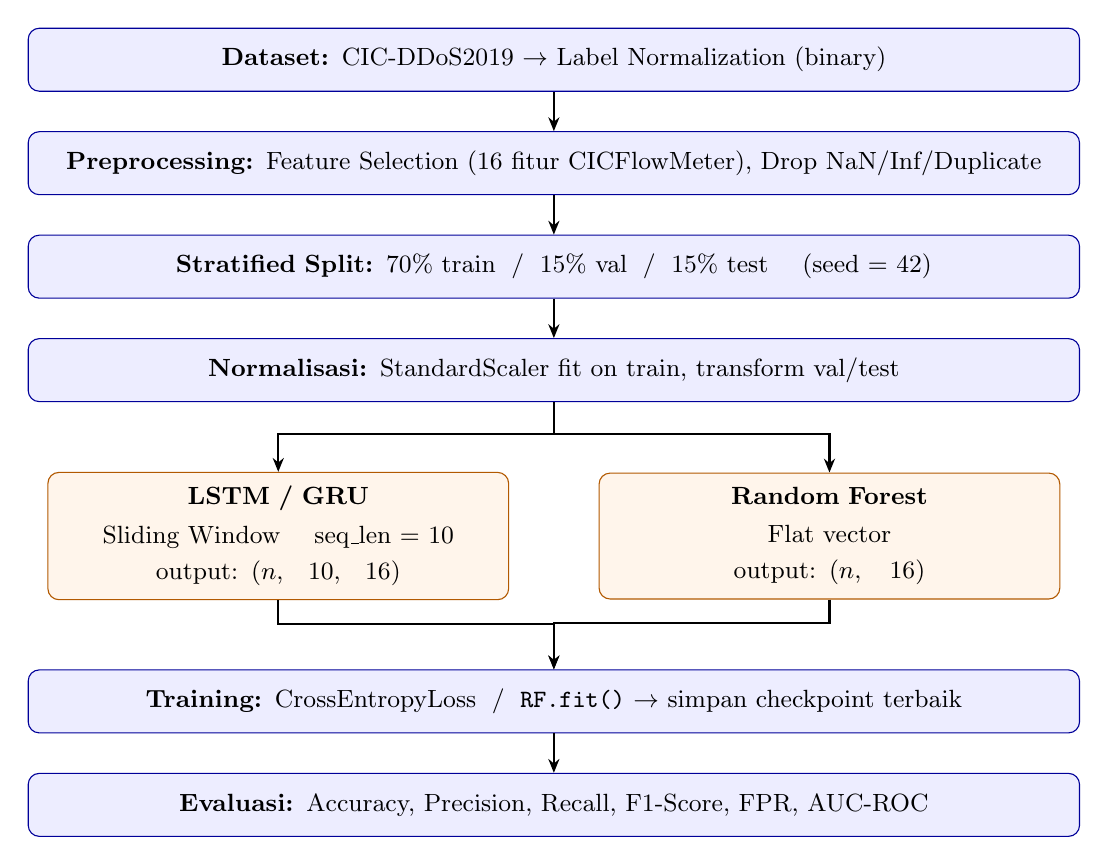
\begin{tikzpicture}[
  node distance=0.5cm,
  proc/.style={rectangle, rounded corners=4pt, draw=blue!60!black,
               fill=blue!7, text width=13cm, align=center,
               minimum height=0.8cm, font=\small, inner sep=5pt},
  branch/.style={rectangle, rounded corners=4pt, draw=orange!70!black,
                 fill=orange!8, text width=5.5cm, align=center,
                 minimum height=1.5cm, font=\small, inner sep=5pt},
  arr/.style={-{Stealth[length=5pt,width=4pt]}, thick}
]
  \node[proc] (D) {\textbf{Dataset:} CIC-DDoS2019 $\to$ Label Normalization (binary)};
  \node[proc, below=of D] (F) {\textbf{Preprocessing:} Feature Selection (16 fitur CICFlowMeter), Drop NaN/Inf/Duplicate};
  \node[proc, below=of F] (S) {\textbf{Stratified Split:} 70\% train \;/\; 15\% val \;/\; 15\% test \quad (seed = 42)};
  \node[proc, below=of S] (N) {\textbf{Normalisasi:} StandardScaler fit on train, transform val/test};
  \node[branch] (L) at ($(N.south)+(-3.5cm,-1.7cm)$) {
    \textbf{LSTM / GRU}\\[3pt]
    Sliding Window \quad seq\_len = 10\\[2pt]
    output: $(n,\;10,\;16)$
  };
  \node[branch] (R) at ($(N.south)+(+3.5cm,-1.7cm)$) {
    \textbf{Random Forest}\\[3pt]
    Flat vector\\[2pt]
    output: $(n,\;16)$
  };
  \node[proc] (T) at ($(N.south)+(0,-3.8cm)$) {\textbf{Training:} CrossEntropyLoss \;/\; \texttt{RF.fit()} $\to$ simpan checkpoint terbaik};
  \node[proc, below=of T] (E) {\textbf{Evaluasi:} Accuracy, Precision, Recall, F1-Score, FPR, AUC-ROC};
  \draw[arr] (D) -- (F);
  \draw[arr] (F) -- (S);
  \draw[arr] (S) -- (N);
  \draw[arr] (N.south) -- ++(0,-0.4) -| (L.north);
  \draw[arr] (N.south) -- ++(0,-0.4) -| (R.north);
  \draw[arr] (L.south) -- ++(0,-0.3) -| (T.north);
  \draw[arr] (R.south) -- ++(0,-0.3) -| (T.north);
  \draw[arr] (T) -- (E);
\end{tikzpicture}
\caption{Block diagram sistem klasifikasi DDoS end-to-end}
\label{fig:block-diagram}
\end{figure}

\section{\textit{Flowchart} Program}

\begin{figure}[H]
\centering
\scalebox{0.88}{%
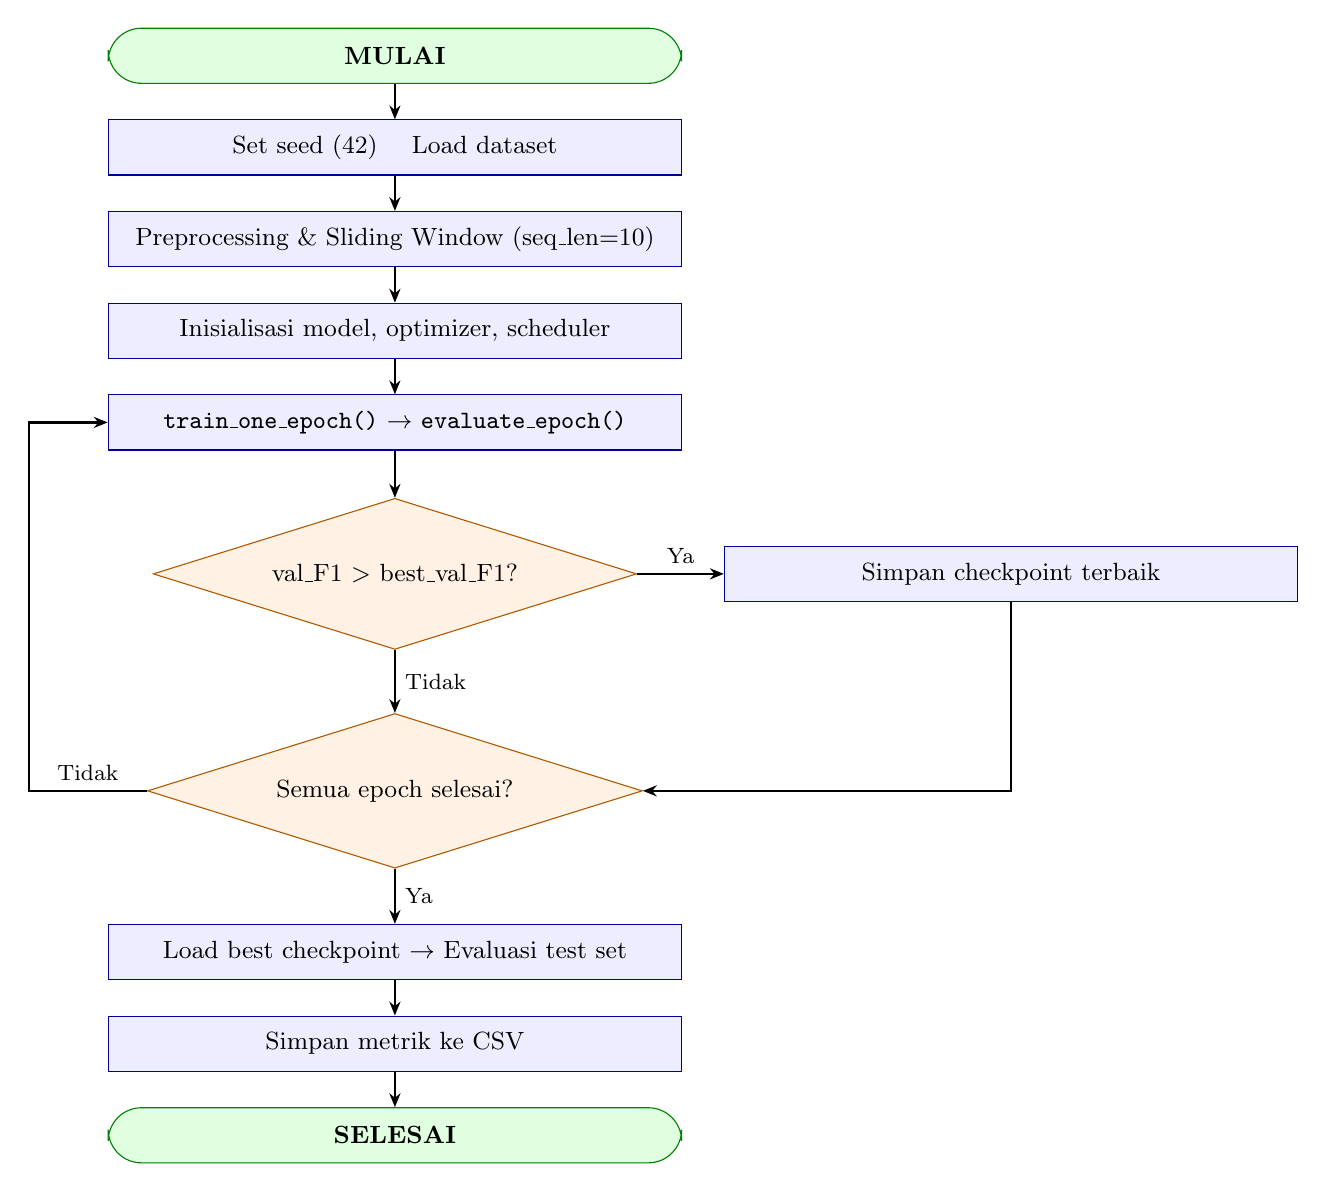
\begin{tikzpicture}[
  node distance=0.45cm,
  startstop/.style={rectangle, rounded corners=12pt, draw=green!50!black,
                    fill=green!12, text width=7cm, align=center,
                    minimum height=0.7cm, font=\small\bfseries, inner sep=4pt},
  proc/.style={rectangle, draw=blue!60!black, fill=blue!7,
               text width=7cm, align=center,
               minimum height=0.7cm, font=\small, inner sep=4pt},
  dec/.style={diamond, aspect=3.2, draw=orange!70!black, fill=orange!10,
              text width=4.5cm, align=center, font=\small, inner sep=3pt},
  arr/.style={-{Stealth[length=5pt,width=4pt]}, thick}
]
  \node[startstop] (start) {MULAI};
  \node[proc, below=of start]  (seed)  {Set seed (42) \quad Load dataset};
  \node[proc, below=of seed]   (pre)   {Preprocessing \& Sliding Window (seq\_len=10)};
  \node[proc, below=of pre]    (init)  {Inisialisasi model, optimizer, scheduler};
  \node[proc, below=of init]   (train) {\texttt{train\_one\_epoch()} $\to$ \texttt{evaluate\_epoch()}};
  \node[dec,  below=0.6cm of train] (chk) {val\_F1 $>$ best\_val\_F1?};
  \node[proc, right=1.1cm of chk]  (save) {Simpan checkpoint terbaik};
  \node[dec,  below=0.8cm of chk]  (done) {Semua epoch selesai?};
  \node[proc, below=0.7cm of done] (load) {Load best checkpoint $\to$ Evaluasi test set};
  \node[proc, below=of load]       (csv)  {Simpan metrik ke CSV};
  \node[startstop, below=of csv]   (end)  {SELESAI};

  \draw[arr] (start) -- (seed);
  \draw[arr] (seed)  -- (pre);
  \draw[arr] (pre)   -- (init);
  \draw[arr] (init)  -- (train);
  \draw[arr] (train) -- (chk);
  \draw[arr] (chk)   -- node[above, font=\footnotesize]{Ya} (save);
  \draw[arr] (save)  |- (done);
  \draw[arr] (chk)   -- node[right, font=\footnotesize]{Tidak} (done);
  \draw[arr] (done.west) -- ++(-1.5,0) node[midway, above, font=\footnotesize]{Tidak}
             |- (train.west);
  \draw[arr] (done)  -- node[right, font=\footnotesize]{Ya} (load);
  \draw[arr] (load)  -- (csv);
  \draw[arr] (csv)   -- (end);
\end{tikzpicture}}
\caption{Flowchart program training LSTM/GRU (RF menggunakan \texttt{fit()} langsung tanpa loop epoch)}
\label{fig:flowchart}
\end{figure}

%==============================================================================
% BAB III - IMPLEMENTASI & HASIL EKSPERIMEN
%==============================================================================
\chapter{IMPLEMENTASI \& HASIL EKSPERIMEN}
\label{bab:implementasi}

\section{Dataset \& Pra-pemrosesan}

\textbf{Sumber dataset:} CIC-DDoS2019 versi \textit{cleaned} dari Kaggle (\url{https://www.kaggle.com/datasets/dhoogla/cicddos2019}), yang merupakan versi yang sudah dibersihkan dari masalah kualitas data pada CSV orisinal CIC-UNB~\cite{sharafaldin2019}: nilai \texttt{Inf} akibat \textit{zero-duration flow} (pembagian dengan nol dalam CICFlowMeter), nilai null, duplikat masif (8 GB $\to$ 910 MB setelah \textit{cleaning}), dan kolom identifier yang berpotensi menyebabkan \textit{data leakage}.

\textbf{Statistik dataset:}
\begin{itemize}[leftmargin=*]
    \item Total sampel: 431.371 baris
    \item Label awal: \texttt{BENIGN} dan 17 jenis serangan DDoS (\texttt{DrDoS\_DNS}, \texttt{DrDoS\_LDAP}, \texttt{DrDoS\_MSSQL}, \texttt{DrDoS\_NetBIOS}, \texttt{DrDoS\_NTP}, \texttt{DrDoS\_SNMP}, \texttt{DrDoS\_SSDP}, \texttt{DrDoS\_UDP}, \texttt{Syn}, \texttt{TFTP}, \texttt{UDP-lag}, dll.)
    \item Label setelah binary mapping: \texttt{normal} ($\approx$97.831 sampel) dan \texttt{ddos} ($\approx$333.540 sampel)
    \item Ketidakseimbangan kelas ditangani dengan \texttt{class\_weight=`balanced'} untuk RF dan \textit{weighted CrossEntropyLoss} untuk LSTM/GRU
\end{itemize}

\textbf{Contoh representatif aliran jaringan:}
\begin{table}[h!]
\centering
\caption{Contoh nilai fitur untuk aliran normal dan DDoS}
\label{tab:contoh-sampel}
\begin{tabular}{lrr}
\toprule
\textbf{Fitur} & \textbf{Normal (BENIGN)} & \textbf{DDoS (DrDoS\_UDP)} \\
\midrule
Flow Duration ($\mu$s)         & 4.512.043 & 42 \\
Total Fwd Packets              & 18        & 1 \\
Total Backward Packets         & 14        & 0 \\
Flow Packets/s                 & 7,1       & 23.809,5 \\
Flow Bytes/s                   & 1.823,4   & 1.428.571,4 \\
Fwd IAT Mean ($\mu$s)         & 282.003   & 0 \\
SYN Flag Count                 & 1         & 0 \\
ACK Flag Count                 & 13        & 0 \\
\bottomrule
\end{tabular}
\end{table}

\textbf{Pembagian dataset:}

\begin{table}[h!]
\centering
\caption{Pembagian dataset (stratified, seed=42)}
\label{tab:split-data}
\begin{tabular}{lrr}
\toprule
\textbf{Subset} & \textbf{Jumlah Sampel} & \textbf{Rasio (\%)} \\
\midrule
Training   & 301.960 & 70\% \\
Validation & 64.706  & 15\% \\
Test       & 64.705  & 15\% \\
\midrule
\textbf{Total} & \textbf{431.371} & \textbf{100\%} \\
\bottomrule
\end{tabular}
\end{table}

\textbf{Pipeline pra-pemrosesan} (diimplementasikan dalam \texttt{src/preprocessing.py}):
\begin{enumerate}[leftmargin=*]
    \item Load semua file Parquet dan normalisasi nama label ke binary (\texttt{normal}/\texttt{ddos})
    \item Seleksi 16 fitur CICFlowMeter yang relevan secara temporal (Flow Duration, Fwd/Bwd packet count/length, Flow Packets/s, Flow Bytes/s, IAT mean, flag counts, average packet size)
    \item Eliminasi baris dengan nilai NaN atau Inf
    \item Stratified 70/15/15 split (seed 42) untuk menjaga proporsi kelas di setiap subset
    \item StandardScaler di-\textit{fit} pada \textit{train set} saja, kemudian ditransformasi ke val dan test (mencegah \textit{data leakage})
    \item \textit{Sliding window} (seq\_len=10, \textit{stride}=1) untuk LSTM/GRU: menghasilkan tensor berukuran $(n, 10, 16)$
    \item \textit{Flat feature vector} untuk Random Forest: menghasilkan array $(n, 16)$
\end{enumerate}

\section{Konfigurasi Eksperimen}

\begin{table}[h!]
\centering
\caption{Konfigurasi hyperparameter eksperimen terbaik per model}
\label{tab:hyperparam}
\begin{tabular}{llll}
\toprule
\textbf{Hyperparameter} & \textbf{LSTM terbaik} & \textbf{GRU terbaik} & \textbf{RF terbaik} \\
\midrule
Hidden size / n\_estimators & 128         & 256         & 100 \\
Num layers / max\_depth     & 2           & 2           & None \\
Dropout                     & 0.3         & 0.3         & -- \\
Seq\_len                    & 10          & 10          & -- \\
Learning rate               & 1e-3        & 1e-3        & -- \\
Batch size                  & 32          & 32          & -- \\
Epochs                      & 50          & 50          & -- \\
Optimizer                   & Adam        & Adam        & -- \\
Scheduler                   & ReduceLROnPlateau & ReduceLROnPlateau & -- \\
Loss function               & Weighted CrossEntropyLoss & Weighted CrossEntropyLoss & -- \\
class\_weight               & --          & --          & balanced \\
Random seed                 & 42          & 42          & 42 \\
Hardware                    & \multicolumn{3}{c}{Google Colab GPU T4} \\
Framework                   & PyTorch 2.x & PyTorch 2.x & scikit-learn 1.x \\
\bottomrule
\end{tabular}
\end{table}

\section{Metrik Evaluasi}

Metrik yang digunakan pada proyek ini dipilih berdasarkan konteks \textit{Intrusion Detection System} (IDS), di mana dua jenis kesalahan memiliki konsekuensi yang berbeda:

\begin{itemize}[leftmargin=*]
    \item \textbf{Accuracy}: proporsi prediksi benar dari seluruh sampel
    \item \textbf{Precision} (DDoS): $\text{TP} / (\text{TP} + \text{FP})$, relevansi \textit{alert} yang diberikan sistem
    \item \textbf{Recall} (DDoS): $\text{TP} / (\text{TP} + \text{FN})$, kemampuan mendeteksi semua serangan (\textit{detection rate})
    \item \textbf{F1-score} (DDoS): \textit{harmonic mean} dari Precision dan Recall
    \item \textbf{FPR} (\textit{False Positive Rate}): $\text{FP} / (\text{FP} + \text{TN})$, lalu lintas normal yang salah diklasifikasikan sebagai serangan; metrik kritis karena FPR tinggi akan membanjiri tim SOC dengan \textit{false alert}
    \item \textbf{AUC-ROC}: luas di bawah kurva ROC; mengukur kemampuan diskriminasi model secara keseluruhan di berbagai ambang batas klasifikasi
\end{itemize}

F1-score dipilih sebagai metrik utama (bukan accuracy) karena ketidakseimbangan kelas yang signifikan (rasio DDoS:Normal $\approx$ 3,4:1).

\section{Hasil Kuantitatif}

\begin{table}[h!]
\centering
\caption{Hasil evaluasi pada \textit{test set} (15\% dari 431.371 sampel)}
\label{tab:hasil-utama}
\begin{tabular}{lcccccc}
\toprule
\textbf{Model} & \textbf{Accuracy} & \textbf{Precision} & \textbf{Recall} & \textbf{F1} & \textbf{FPR} & \textbf{AUC} \\
\midrule
LSTM (hidden=128, layers=2) & 99,63\% & 99,87\% & 99,65\% & 0,9976 & 0,46\% & 0,9996 \\
GRU  (hidden=256, layers=2) & 99,61\% & 99,92\% & 99,58\% & 0,9975 & 0,28\% & 0,9996 \\
Random Forest (n\_est=100)  & 99,87\% & 99,96\% & 99,88\% & 0,9992 & 0,15\% & 0,9998 \\
\bottomrule
\end{tabular}
\end{table}

Ketiga model mencapai performa yang sangat tinggi. Perbedaan F1-score absolut antara model terbaik (RF: 0,9992) dan terburuk (GRU: 0,9975) hanya 0,0017. Namun dari perspektif operasional IDS, perbedaan FPR antara RF (0,15\%) dan LSTM (0,46\%) cukup signifikan: pada volume lalu lintas 10 juta paket normal per hari, FPR 0,46\% menghasilkan 46.000 \textit{false alert} per hari, sementara FPR 0,15\% menghasilkan 15.000, selisih 31.000 \textit{false alert} yang harus ditangani tim SOC.

\begin{figure}[h!]
\centering
\begin{subfigure}[t]{0.3\textwidth}
    \centering
    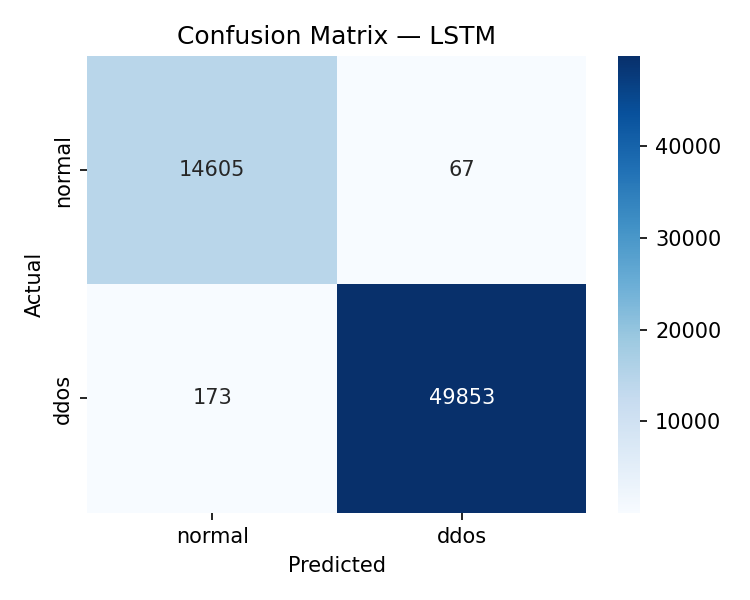
\includegraphics[width=\textwidth]{cm_lstm.png}
    \caption{LSTM}
\end{subfigure}
\hfill
\begin{subfigure}[t]{0.3\textwidth}
    \centering
    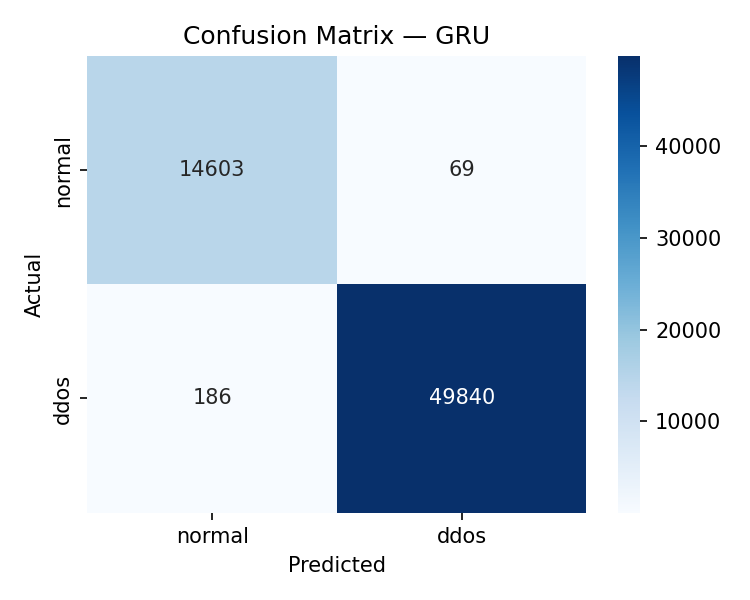
\includegraphics[width=\textwidth]{cm_gru.png}
    \caption{GRU}
\end{subfigure}
\hfill
\begin{subfigure}[t]{0.3\textwidth}
    \centering
    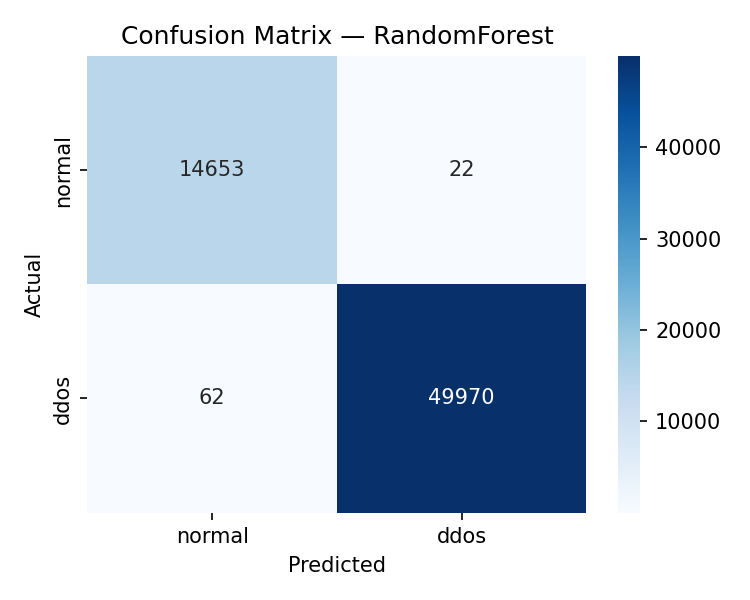
\includegraphics[width=\textwidth]{cm_randomforest.png}
    \caption{Random Forest}
\end{subfigure}
\caption{Confusion matrix ketiga model pada \textit{test set}}
\label{fig:confusion-matrices}
\end{figure}

\begin{figure}[h!]
\centering
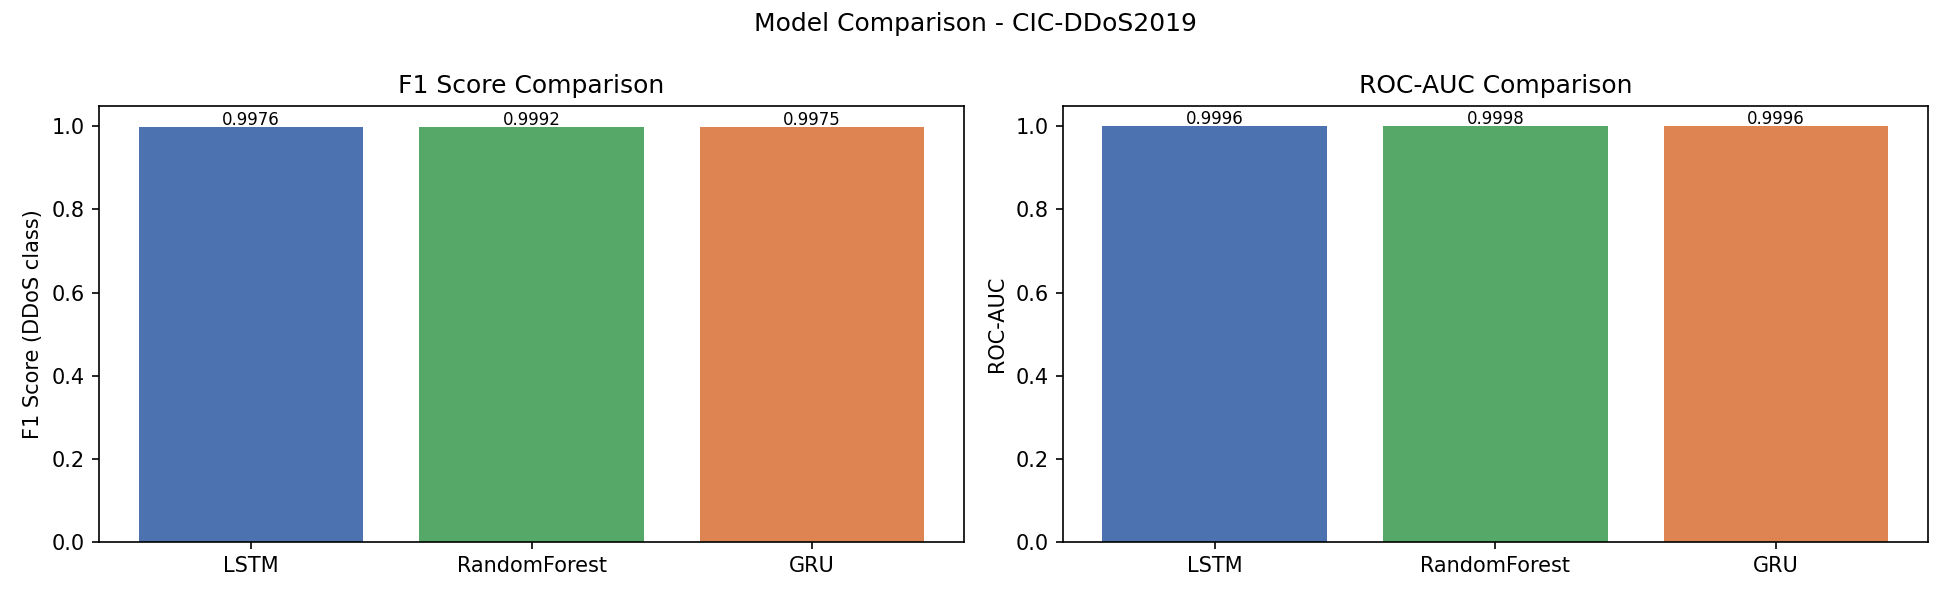
\includegraphics[width=0.75\textwidth]{model_comparison_bar.png}
\caption{Perbandingan metrik utama ketiga model}
\label{fig:model-comparison}
\end{figure}

\section{Analisis \textit{Hyperparameter Tuning}}

\begin{table}[h!]
\centering
\caption{Dokumentasi eksperimen LSTM (50 epoch, batch=32, lr=1e-3 kecuali disebutkan)}
\label{tab:lstm-tuning}
\begin{tabular}{lcccccc}
\toprule
\textbf{Exp ID} & \textbf{hidden} & \textbf{layers} & \textbf{dropout} & \textbf{seq\_len} & \textbf{Val F1} & \textbf{Catatan} \\
\midrule
lstm\_01 & 128 & 2 & 0.3 & 10 & 0.9976 & Baseline (dipilih) \\
lstm\_02 & 64  & 2 & 0.3 & 10 & 0.9977 & hidden lebih kecil \\
lstm\_03 & 256 & 2 & 0.3 & 10 & 0.9975 & hidden lebih besar \\
lstm\_04 & 128 & 3 & 0.3 & 10 & 0.9976 & layer tambahan \\
lstm\_05 & 128 & 2 & 0.5 & 10 & 0.9974 & dropout lebih tinggi \\
lstm\_06 & 128 & 2 & 0.3 & 5  & 0.9974 & window lebih pendek \\
\bottomrule
\end{tabular}
\end{table}

\begin{table}[h!]
\centering
\caption{Dokumentasi eksperimen GRU (50 epoch, batch=32, seq\_len=10 kecuali disebutkan)}
\label{tab:gru-tuning}
\begin{tabular}{lcccccc}
\toprule
\textbf{Exp ID} & \textbf{hidden} & \textbf{layers} & \textbf{dropout} & \textbf{lr} & \textbf{Val F1} & \textbf{Catatan} \\
\midrule
gru\_01 & 128 & 2 & 0.3 & 1e-3 & 0.9975 & Baseline \\
gru\_02 & 64  & 2 & 0.3 & 1e-3 & 0.9975 & hidden lebih kecil \\
gru\_03 & 256 & 2 & 0.3 & 1e-3 & 0.9976 & hidden lebih besar (best val) \\
gru\_04 & 128 & 3 & 0.3 & 1e-3 & 0.9973 & layer tambahan \\
gru\_05 & 128 & 2 & 0.3 & 1e-4 & 0.9971 & lr lebih rendah \\
gru\_06 & 128 & 2 & 0.5 & 1e-3 & 0.9973 & dropout lebih tinggi \\
\bottomrule
\end{tabular}
\end{table}

\begin{table}[h!]
\centering
\caption{Dokumentasi eksperimen Random Forest}
\label{tab:rf-tuning}
\begin{tabular}{lccccc}
\toprule
\textbf{Exp ID} & \textbf{n\_estimators} & \textbf{max\_depth} & \textbf{min\_samples\_split} & \textbf{Val F1} & \textbf{Catatan} \\
\midrule
rf\_01 & 100 & None & 2 & 0.9990 & Baseline (dipilih) \\
rf\_02 & 50  & None & 2 & 0.9990 & tree lebih sedikit \\
rf\_03 & 200 & None & 2 & 0.9990 & tree lebih banyak \\
rf\_04 & 100 & 10   & 2 & 0.9980 & kedalaman dibatasi \\
rf\_05 & 100 & 20   & 2 & 0.9990 & kedalaman sedang \\
rf\_06 & 100 & None & 5 & 0.9989 & min\_split lebih besar \\
\bottomrule
\end{tabular}
\end{table}

Temuan dari tuning: (1) LSTM dan GRU sangat tidak sensitif terhadap perubahan \textit{hidden\_size} dan \textit{num\_layers} dalam rentang yang diuji; semua konfigurasi menghasilkan Val F1 dalam rentang 0,9971--0,9977; (2) Random Forest hampir tidak sensitif terhadap \texttt{n\_estimators} (50--200 memberikan hasil yang sama), tetapi \texttt{max\_depth=10} menurunkan performa sedikit, mengindikasikan bahwa \textit{full-depth} diperlukan untuk menangkap batas keputusan yang kompleks; (3) Mengurangi \texttt{seq\_len} dari 10 ke 5 menurunkan Val F1 LSTM dari 0,9976 ke 0,9974, indikasi kecil bahwa konteks 10 timestep lebih informatif.

\section{Hasil Kualitatif \& \textit{Error Analysis}}

Berdasarkan \textit{confusion matrix} pada test set ($\approx$64.705 sampel: $\approx$14.675 normal + $\approx$50.030 DDoS):

\textbf{Jenis kesalahan LSTM (FPR=0,46\%, $\approx$68 FP):}
\begin{itemize}[leftmargin=*]
    \item \textit{False Positive} (normal $\to$ diprediksi DDoS): lalu lintas normal dengan karakteristik mirip DDoS, seperti \textit{burst traffic} dari CDN atau streaming video dengan laju paket tinggi, salah diklasifikasikan. Ini adalah 68 dari 14.675 sampel normal ($\approx$0,46\%).
    \item \textit{False Negative} (DDoS $\to$ diprediksi normal): $\approx$175 sampel DDoS tidak terdeteksi, kemungkinan besar berasal dari serangan \textit{low-rate} seperti \texttt{UDP-lag} yang memiliki karakteristik mendekati lalu lintas normal.
\end{itemize}

\textbf{Jenis kesalahan GRU (FPR=0,28\%, $\approx$41 FP):} GRU memiliki FPR lebih rendah dari LSTM tetapi Recall sedikit lebih rendah (99,58\% vs.\ 99,65\%), mengindikasikan bahwa GRU lebih "konservatif" dalam memberikan label DDoS.

\textbf{Jenis kesalahan RF (FPR=0,15\%, $\approx$22 FP):} RF menghasilkan kesalahan paling sedikit di kedua jenis (FP dan FN), dikuatkan oleh AUC tertinggi (0,9998). Fitur CICFlowMeter yang sudah ter-\textit{engineer} memberikan representasi yang kaya untuk pohon keputusan.

\textbf{Hipotesis penyebab kegagalan:}
\begin{enumerate}[leftmargin=*]
    \item \textit{Burst traffic} yang sah (CDN \textit{prefetch}, streaming video, backup) memiliki statistik \textit{inter-arrival time} dan laju paket yang tumpang tindih dengan DDoS volumetrik, menyebabkan FP.
    \item Serangan \textit{low-rate} (mis.\ \texttt{UDP-lag}) dirancang untuk menyerupai lalu lintas normal; model apapun kesulitan mengklasifikasikannya tanpa konteks traffic jangka panjang.
    \item Fitur CICFlowMeter sudah merupakan agregasi statistik per aliran (bukan urutan paket mentah), sehingga "temporal information" yang ingin dieksploitasi LSTM sudah terabstraksi ke dalam fitur-fitur tersebut, menjelaskan mengapa pemodelan sekuensial tidak memberikan keunggulan atas RF.
\end{enumerate}

\section{Pembahasan}

\subsection*{III.7.1 Interpretasi terhadap Rumusan Masalah}

\textbf{RM1 (Performa LSTM):} LSTM mencapai F1-score 0,9976 dan FPR 0,46\% pada test set, performa yang sangat baik untuk sistem deteksi intrusi. Jauh melampaui threshold praktis yang umum digunakan dalam literature ($>$99\% recall untuk DDoS detection).

\textbf{RM2 (Perbandingan LSTM vs.\ GRU vs.\ RF):} Hipotesis awal bahwa LSTM akan mengungguli GRU dan RF tidak terkonfirmasi. Urutan performa: RF $>$ LSTM $>$ GRU. Penjelasan: dataset CIC-DDoS2019 menggunakan fitur CICFlowMeter yang sudah merupakan statistik agregat per-aliran, bukan urutan paket mentah. Temporal information yang menjadi keunggulan LSTM/GRU sudah terabstraksi ke dalam fitur-fitur ini, sehingga RF yang secara inheren mengeksploitasi kombinasi fitur tabular mampu berkinerja lebih baik. Temuan ini konsisten dengan literatur yang menunjukkan bahwa pada dataset dengan \textit{hand-crafted features} yang kuat, model ML tradisional sering kompetitif dengan deep learning.

\textbf{RM3 (Pengaruh hyperparameter):} LSTM dan GRU sangat robust terhadap perubahan hyperparameter dalam rentang yang diuji (Val F1 bervariasi $<$0,0007). RF paling sensitif terhadap \texttt{max\_depth}: pembatasan kedalaman (\texttt{depth=10}) menurunkan performa sebesar 0,001 Val F1.

\subsection*{III.7.2 Analisis Etika, Bias, dan Keterbatasan (Bonus B3)}

\textbf{1. Distribusi shift lab-ke-produksi:} CIC-DDoS2019 ditangkap dalam lingkungan testbed terkontrol di University of New Brunswick dengan konfigurasi jaringan spesifik. Traffic ISP produksi memiliki distribusi yang berbeda secara fundamental: base rate serangan yang lebih rendah, noise yang lebih tinggi, dan campuran protokol yang lebih beragam. Model yang dilatih pada CIC-DDoS2019 berpotensi memiliki FPR yang jauh lebih tinggi di lingkungan produksi karena distribusi lalu lintas normal yang berbeda.

\textbf{2. Temporal drift:} Dataset diambil pada 2019. Lanskap serangan DDoS telah berkembang signifikan: serangan berbasis QUIC, HTTP/2 RST flood, \textit{botnet} IoT generasi baru, dan teknik amplifikasi melalui layanan cloud tidak ada dalam data training. Model yang dilatih pada CIC-DDoS2019 akan gagal mendeteksi serangan-serangan ini dan memerlukan retraining berkala dengan data terbaru.

\textbf{3. Ketidakseimbangan kelas dan bias benchmark:} Dalam CIC-DDoS2019, sampel DDoS mendominasi ($\approx$77\% dari total sampel), yang tidak mencerminkan rasio DDoS:normal pada traffic ISP nyata (di mana serangan jauh lebih jarang). Akibatnya, model yang dilatih pada dataset ini mungkin memiliki Recall yang terlalu optimis dan Precision yang terlalu rendah ketika di-\textit{deploy} pada lingkungan dengan rasio kelas yang berbeda.

\textbf{4. Keterbatasan generalisasi:} Serangan yang dirancang untuk menyerupai lalu lintas normal (\textit{low-rate DDoS}, \textit{application-layer DDoS}) sulit dideteksi oleh model yang dilatih pada serangan volumetrik. Penyerang yang sadar akan adanya model ML dapat melakukan \textit{adversarial traffic shaping} untuk menghindari deteksi.

\textbf{5. Implikasi penggunaan bertanggung jawab:} Model ini seharusnya digunakan sebagai lapisan awal deteksi yang dikombinasikan dengan analisis kontekstual manusia (SOC analyst), bukan sebagai sistem pengambilan keputusan otonom. FPR sebesar 0,15--0,46\% dapat menghasilkan ribuan \textit{false alert} per hari pada jaringan skala besar, yang berpotensi menyebabkan \textit{alert fatigue} dan terlewatnya ancaman nyata.

%==============================================================================
% BAB IV - PEMBAGIAN TUGAS & DEKLARASI KONTRIBUSI INDIVIDUAL
%==============================================================================
\chapter{PEMBAGIAN TUGAS \& DEKLARASI KONTRIBUSI INDIVIDUAL}
\label{bab:kontribusi}

Klaim penguasaan konsep per anggota dideklarasikan dalam berkas \texttt{metadata-laporan-akhir-kel06.json} yang merupakan bagian tidak terpisahkan dari laporan ini.

%-------------------- Anggota 1 -----------------------------------------------
\section{Calvin Wirathama Katoroy -- NPM. 2306242395}

\subsection*{IV.1.1 Komponen yang Dikerjakan}
Daftar konkret bagian proyek yang menjadi tanggung jawab penuh saya:
\begin{itemize}[leftmargin=*]
    \item \textbf{Kode/modul:} \texttt{src/models/lstm\_model.py}, \texttt{src/models/gru\_model.py}, \texttt{src/train.py}, \texttt{config.yaml}
    \item \textbf{Bagian arsitektur:} Desain LSTM dan GRU classifier (pilihan hidden\_size, num\_layers, dropout, classification head Linear(128$\to$64, ReLU, Dropout)$\to$Linear(64$\to$2)), training loop dengan logging per epoch, weighted loss untuk class imbalance, AMP (Automatic Mixed Precision) untuk efisiensi GPU
    \item \textbf{Bagian analisis:} Justifikasi pemilihan LSTM vs.\ GRU, rancangan hyperparameter grid, koneksi dengan penelitian GANDD-Bridge Network Lab DTE FT UI, analisis trade-off seq\_len vs.\ computational cost
    \item \textbf{Bagian laporan:} Bab I, Bab II.2 (landasan teori LSTM/GRU), Bab II.3 (justifikasi), Bab III.3, Bab III.5 (tuning LSTM \& GRU), Bab III.7
\end{itemize}

\subsection*{IV.1.2 Pernyataan Penggunaan AI \textit{Assistant}}
\begin{itemize}[leftmargin=*]
    \item \textbf{Tool yang dipakai:} Claude Sonnet 4.6 (Claude Code CLI, Anthropic)
    \item \textbf{Untuk bagian apa:} Debugging sesekali pada training loop (path resolution di Colab, PyTorch AMP deprecation warning) dan pengecekan tata bahasa pada bagian laporan yang saya tulis
    \item \textbf{Tingkat ketergantungan:} rendah
    \item \textbf{Pernyataan:} Saya memahami dan dapat mempertanggungjawabkan setiap baris kode dan teks yang saya klaim sebagai bagian saya.
\end{itemize}

%-------------------- Anggota 2 -----------------------------------------------
\section{Syahmi Hamdani -- NPM. 2306220532}

\subsection*{IV.2.1 Komponen yang Dikerjakan}
Daftar konkret bagian proyek yang menjadi tanggung jawab penuh saya:
\begin{itemize}[leftmargin=*]
    \item \textbf{Kode/modul:} \texttt{src/preprocessing.py}, \texttt{verify\_dataset.py}, \texttt{notebooks/01\_eda.ipynb}, \texttt{notebooks/02\_preprocessing.ipynb}
    \item \textbf{Bagian arsitektur:} Pipeline pra-pemrosesan data (normalisasi label biner, seleksi 16 fitur CICFlowMeter, eliminasi NaN/Inf, stratified 70/15/15 split seed 42, StandardScaler fit pada train set, sliding window $(n, 10, 16)$ untuk LSTM/GRU), skrip validasi integritas dataset splits
    \item \textbf{Bagian analisis:} EDA sebaran kelas (class imbalance), analisis korelasi antar fitur (Pearson correlation heatmap), penentuan 16 fitur temporal kritis dari CICFlowMeter
    \item \textbf{Bagian laporan:} Bab III.1 (Dataset \& Pra-pemrosesan), Bab III.2 (Pembagian Dataset), Lampiran A (Metadata JSON)
\end{itemize}

\subsection*{IV.2.2 Pernyataan Penggunaan AI \textit{Assistant}}
\begin{itemize}[leftmargin=*]
    \item \textbf{Tool yang dipakai:} Gemini (Google), Claude Sonnet 4.6 (Anthropic)
    \item \textbf{Untuk bagian apa:} Debugging sesekali pada preprocessing pipeline (penanganan nilai Inf CICFlowMeter, validasi konsistensi split) dan pengecekan tata bahasa pada bagian laporan yang saya tulis
    \item \textbf{Tingkat ketergantungan:} sedang
    \item \textbf{Pernyataan:} Saya memahami dan dapat mempertanggungjawabkan setiap baris kode dan teks yang saya klaim sebagai bagian saya.
\end{itemize}

%-------------------- Anggota 3 -----------------------------------------------
\section{Christover Angelo -- NPM. 2306220323}

\subsection*{IV.3.1 Komponen yang Dikerjakan}
Daftar konkret bagian proyek yang menjadi tanggung jawab penuh saya:
\begin{itemize}[leftmargin=*]
    \item \textbf{Kode/modul:} \texttt{notebooks/09\_error\_analysis.ipynb}; artefak \texttt{results/figures/cm\_estimated\_comparison.png} dan \texttt{cost\_sensitive\_comparison.png}
    \item \textbf{Bagian arsitektur/eksekusi:} Notebook analisis lanjutan \textbf{read-only} atas hasil \texttt{notebooks/08\_evaluation.ipynb} (\texttt{final\_comparison.csv}, gambar CM); tidak mengubah pipeline training maupun \texttt{metrics\_summary.csv}.
    \item \textbf{Bagian analisis:} \textit{Error analysis} teknis LSTM, GRU, Random Forest: rekonstruksi confusion matrix dari FPR/recall, verifikasi metrik sklearn, \textit{cost-sensitive analysis} ($w_{FN}=10w_{FP}$), interpretasi FP/FN, rekomendasi deploy RF.
    \item \textbf{Bagian laporan:} Bab Hasil Kualitatif \& \textit{Error Analysis}; interpretasi evaluasi; pembahasan perbandingan model.
\end{itemize}

\subsection*{IV.3.2 Pernyataan Penggunaan AI \textit{Assistant}}
\begin{itemize}[leftmargin=*]
    \item \textbf{Tool yang dipakai:} Cursor
    \item \textbf{Untuk bagian apa:} Debugging dan enivironment IDE
    \item \textbf{Pernyataan:} Saya memahami kode, visualisasi, rumus metrik, dan isi analisis yang saya tambahkan sebagai bagian kontribusi individu saya pada proyek ini.
\end{itemize}

%-------------------- Anggota 4 -----------------------------------------------
\section{Matthew Immanuel -- NPM. 2306221024}

\subsection*{IV.4.1 Komponen yang Dikerjakan}
Daftar konkret bagian proyek yang menjadi tanggung jawab penuh saya:
\begin{itemize}[leftmargin=*]
    \item \textbf{Kode/modul:} \texttt{notebooks/05\_rf\_training.ipynb}, \texttt{notebooks/08\_evaluation.ipynb}; manajemen pencatatan pada \texttt{results/metrics\_summary.csv} dan direktori \texttt{results/figures/}
    \item \textbf{Bagian arsitektur/eksekusi:} Menjalankan eksperimen \textit{tuning hyperparameter} model \textit{baseline} Random Forest sebanyak 5 kali iterasi (variasi \texttt{n\_estimators} dan \texttt{max\_depth}) dan mengelola pemuatan (\textit{loading}) \textit{checkpoint} model untuk evaluasi.
    \item \textbf{Bagian analisis:} Mengeksekusi komparasi performa final ketiga arsitektur model (LSTM, GRU, Random Forest), menghasilkan tabel perbandingan, serta membuat visualisasi \textit{Confusion Matrix} dan \textit{ROC Curve overlay}.
    \item \textbf{Bagian laporan:} Desain Eksperimen Baseline, Hasil Evaluasi dan Analisis Komparatif, Kesimpulan Perbandingan Model.
\end{itemize}

\subsection*{IV.4.2 Pernyataan Penggunaan AI \textit{Assistant}}
\begin{itemize}[leftmargin=*]
    \item \textbf{Tool yang dipakai:} Gemini, ChatGPT
    \item \textbf{Untuk bagian apa:} \textit{Debugging} sintaks Python, perbaikan \textit{error} saat memuat \textit{checkpoint} antar-\textit{environment}, dan penyesuaian parameter visualisasi grafik Matplotlib.
    \item \textbf{Pernyataan:} Saya memahami kode dan teks yang saya klaim sebagai bagian saya.
\end{itemize}

%==============================================================================
% BAB V - KESIMPULAN & PEKERJAAN LANJUTAN
%==============================================================================
\chapter{KESIMPULAN \& PEKERJAAN LANJUTAN}
\label{bab:kesimpulan}

\section{Kesimpulan}

\begin{enumerate}[leftmargin=*]
    \item \textbf{(RM1)} Model LSTM mencapai F1-score 0,9976, accuracy 99,63\%, dan AUC 0,9996 pada test set CIC-DDoS2019, menunjukkan kemampuan yang sangat baik dalam mengklasifikasikan lalu lintas jaringan DDoS secara biner, dengan hanya 0,46\% lalu lintas normal yang salah diklasifikasikan sebagai serangan.

    \item \textbf{(RM2)} Hipotesis bahwa LSTM akan mengungguli GRU dan Random Forest tidak terkonfirmasi. Urutan performa pada test set adalah RF (F1=0,9992, FPR=0,15\%) $>$ LSTM (F1=0,9976, FPR=0,46\%) $>$ GRU (F1=0,9975, FPR=0,28\%). Keunggulan RF disebabkan oleh sifat fitur CICFlowMeter yang sudah merupakan statistik agregat aliran, sehingga informasi temporal yang menjadi keunggulan LSTM/GRU sudah terabstraksi ke dalam representasi fitur ini.

    \item \textbf{(RM3)} LSTM dan GRU sangat tidak sensitif terhadap perubahan hyperparameter dalam rentang yang diuji (Val F1 bervariasi $<$0,0007). Hyperparameter yang paling berpengaruh pada RF adalah \texttt{max\_depth}: pembatasan kedalaman menurunkan Val F1 sebesar 0,001. Hasil ini mengindikasikan bahwa performa tinggi pada dataset ini dapat dicapai dengan konfigurasi yang relatif sederhana tanpa tuning intensif.
\end{enumerate}

\section{Klaim Bonus Skor}

\begin{itemize}[leftmargin=*]
    \item[$\checkmark$] \textbf{B1. Evaluasi Komparatif \& Iterasi:} Tiga model (LSTM, GRU, RF) dibandingkan pada dataset dan metrik yang seragam. Terdokumentasi 6 eksperimen LSTM (Tabel \ref{tab:lstm-tuning}), 6 eksperimen GRU (Tabel \ref{tab:gru-tuning}), dan 6 eksperimen RF (Tabel \ref{tab:rf-tuning}), dengan analisis sensitivitas hyperparameter.
    \item[$\square$] \textbf{B2. Dataset Mandiri:} Tidak diklaim; menggunakan CIC-DDoS2019 (dataset benchmark publik) untuk reliabilitas hasil dan reprodusibilitas.
    \item[$\checkmark$] \textbf{B3. Analisis Etika, Bias, \& Keterbatasan:} Dibahas pada Subbab \ref{bab:implementasi}.7.2, mencakup distribusi shift lab-ke-produksi, temporal drift, bias ketidakseimbangan kelas, keterbatasan generalisasi, dan implikasi penggunaan bertanggung jawab.
\end{itemize}

\section{Pekerjaan Lanjutan (\textit{Future Work})}

\begin{enumerate}[leftmargin=*]
    \item Mengevaluasi model pada dataset lalu lintas jaringan yang lebih baru (mis.\ CIC-DDoS2023, atau dataset yang ditangkap dari ISP produksi) untuk mengkuantifikasi \textit{temporal drift} dan degradasi performa.
    \item Mengganti input dari fitur CICFlowMeter agregat ke urutan \textit{raw packet features} untuk menguji apakah LSTM memang unggul ketika data benar-benar bersifat sekuensial (bukan agregasi).
    \item Mengintegrasikan model terbaik (RF) sebagai komponen klasifikasi dalam pipeline GANDD-Bridge di Wazuh SIEM dan membandingkan performa \textit{end-to-end} dengan sistem berbasis RF yang sudah ada.
    \item Menambahkan modul interpretability (mis.\ SHAP values untuk RF, attention visualization untuk LSTM) untuk memahami fitur mana yang paling berkontribusi pada keputusan klasifikasi.
    \item Mengevaluasi robustness model terhadap \textit{adversarial traffic shaping}, yaitu apakah penyerang yang mengetahui arsitektur model dapat memodifikasi pola serangannya untuk menghindari deteksi.
\end{enumerate}

%==============================================================================
% DAFTAR PUSTAKA
%==============================================================================
\printbibliography[heading=bibintoc,title={DAFTAR PUSTAKA}]

%==============================================================================
% LAMPIRAN
%==============================================================================
\appendix
\renewcommand{\thechapter}{\Alph{chapter}}
\titleformat{\chapter}[display]
  {\normalfont\Large\bfseries\centering}
  {\appendixname\ \thechapter}{12pt}{\Large}

%------ Lampiran A: Metadata JSON --------------------------------------------
\chapter{Berkas Metadata Proyek (JSON)}
\label{lamp:metadata}

Berikut adalah isi berkas \texttt{metadata-laporan-akhir-kel06.json} yang dikumpulkan bersama laporan ini.

\begin{lstlisting}[language=json]
{
  "kode_kelompok": "K06",
  "topik_pilihan": 2,
  "nama_topik": "RNN / GRU / LSTM",
  "judul_proyek": "Klasifikasi Lalu Lintas Jaringan DDoS Menggunakan LSTM,
                   GRU, dan Random Forest pada Dataset CIC-DDoS2019",
  "metode_ai": [
    {"nama": "LSTM", "peran": "utama"},
    {"nama": "GRU",  "peran": "baseline"},
    {"nama": "Random Forest", "peran": "baseline"}
  ],
  "datasets": [{
    "nama": "CIC-DDoS2019 (Kaggle cleaned)",
    "tipe": "publik",
    "url_sumber_publik": "https://www.kaggle.com/datasets/dhoogla/cicddos2019",
    "jumlah_sampel": 431371,
    "jumlah_kelas": 2
  }],
  "klaim_bonus": ["B1", "B3"],
  "tautan": {
    "github": "https://github.com/calvinkatoroy/tugas-akhir-ai-kel-06",
    "colab": "https://colab.research.google.com/drive/1rhoLvdyzKTdK9sGd4dRjkglO-lo2bBHB"
  }
}
\end{lstlisting}

%------ Lampiran B: Tautan Repositori ----------------------------------------
\chapter{Tautan Repositori \& Sumber}
\label{lamp:tautan}

\newcommand{\nburl}[1]{\url{https://colab.research.google.com/github/calvinkatoroy/tugas-akhir-ai-kel-06/blob/master/notebooks/#1}}

\begin{description}[leftmargin=5.5cm,labelwidth=5cm, font=\small]
    \item[GitHub repo:] \url{https://github.com/calvinkatoroy/tugas-akhir-ai-kel-06}
    \item[Google Drive (data):] \url{https://drive.google.com/drive/folders/1zMA2zvF8X0YFK6aUMIFcxZS61SwtzHnX?usp=drive_link}
    \item[Colab -- EDA:] \nburl{01\_eda.ipynb}
    \item[Colab -- Preprocessing:] \nburl{02\_preprocessing.ipynb}
    \item[Colab -- LSTM Training:] \nburl{03\_lstm\_training.ipynb}
    \item[Colab -- GRU Training:] \nburl{04\_gru\_training.ipynb}
    \item[Colab -- RF Training:] \nburl{05\_rf\_training.ipynb}
    \item[Colab -- Evaluation:] \nburl{08\_evaluation.ipynb}
    \item[Colab -- Error Analysis:] \nburl{09\_error\_analysis.ipynb}
    \item[Colab -- Demo (Gradio):] \nburl{demo.ipynb}
    \item[Dataset (Kaggle):] \url{https://www.kaggle.com/datasets/dhoogla/cicddos2019}
    \item[Dataset asli (CIC):] \url{https://www.unb.ca/cic/datasets/ddos-2019.html}
    \item[Video demo:] (terlampir terpisah / dikumpulkan via EMAS)
\end{description}

\textbf{Status akses:} repositori dan folder Drive bersifat publik; seluruh tautan Colab dapat dibuka tanpa login. Sudah diverifikasi terbuka per 25 Mei 2026.

\vspace{0.8em}
\noindent\textbf{Cara menjalankan notebook di Google Colab:}
\begin{enumerate}[leftmargin=*, itemsep=0.2em]
    \item Buka tautan Google Drive di atas dan klik \textbf{Add shortcut to Drive} $\to$ pilih \textbf{My Drive} (root). Pastikan nama shortcut adalah \texttt{tugas-akhir-ai} (sesuai nama folder asli).
    \item Buka salah satu tautan Colab di atas. Pastikan runtime menggunakan \textbf{GPU} (\textit{Runtime} $\to$ \textit{Change runtime type} $\to$ T4 GPU).
    \item Jalankan semua cell secara berurutan (\textit{Runtime} $\to$ \textit{Run all}). Cell mount Drive akan meminta izin akses; klik \textit{Allow}.
    \item Data splits, model checkpoint, dan hasil evaluasi dibaca/ditulis ke \texttt{/content/drive/MyDrive/tugas-akhir-ai/} secara otomatis.
\end{enumerate}

%------ Lampiran C: Research Participation Consent Form ----------------------
\renewcommand{\appendixname}{APPENDIX}

\chapter{Research Participation Consent Form (\textit{Informed Consent})}
\label{lamp:consent}

{\small
\textbf{C.1\quad Brief Explanation.}
\textit{Research:} Development \& validation of an \textit{agentic AI} framework for supporting academic oral examinations.
\textit{Principal investigator:} Muhammad Firdaus Syawaludin Lubis, Ph.D., Department of Computer Engineering, Universitas Indonesia.
\textit{Context:} data collection is conducted alongside the oral examination of the AI course's final assessment.

\textbf{C.2\quad Data Collected.}
Final report (PDF) and \texttt{metadata.json}; audio and video recordings of the oral examination; automatic transcripts; lecturer's judgment scores and AI system's judgment scores.

\textbf{C.3\quad Data Management.}
Participant names and NPMs will be anonymized (replaced with participant codes). Publications will not contain individual identities. Data is stored encrypted; retention is 5 years after the research concludes.

\textbf{C.4\quad Participant Rights.}
(1) Right to decline without affecting the course grade. (2) Right to partial participation. (3) Right to withdraw data until 30 June 2026. (4) Right to ask questions. (5) Right to receive a summary of findings.

\textbf{C.5\quad Individual Consent.}
Each member completes their personal block below. Tick \textbf{exactly one} option (A / B / C) and sign.
}

%--- Member 1: Calvin Wirathama Katoroy ---
\newpage
\section*{Individual Consent: Calvin Wirathama Katoroy}

\noindent
\begin{tabular}{p{0.28\textwidth}p{0.65\textwidth}}
Full name        & : Calvin Wirathama Katoroy \\
Student ID (NPM) & : 2306242395 \\
Email            & : calvinwkatoroy@gmail.com \\
\end{tabular}

\vspace{1.5em}

I have read Sections C.1--C.4 and understood their contents. I voluntarily choose the following option:

\vspace{0.5em}

\begin{itemize}[leftmargin=2em, itemsep=0.8em]
    \item[$\boxtimes$] \textbf{Option A: Full Participation.} I consent to the use of my report, metadata, \textbf{and} the audio and video recordings of my oral examination for research purposes.
    \item[$\square$] \textbf{Option B: Limited Participation.} I consent to the use of my report, metadata, and audio recording, \textbf{but I do not consent to the video recording} being used for research.
    \item[$\square$] \textbf{Option C: Decline Participation.} I decline to participate in the research.
\end{itemize}

\vfill

\noindent
\begin{tabular}{p{0.45\textwidth}p{0.45\textwidth}}
\centering Participant's signature & \centering Witness / researcher's signature \tabularnewline[0.3cm]
\centering 
\includegraphics[width=3.5cm]{calvin_signature.png} & \centering \tabularnewline[0.5cm]
\centering (Calvin Wirathama Katoroy) & \centering (\hspace{4cm}) \tabularnewline
\centering Date: 25 Mei 2026 & \centering Date: \hspace{3cm} \tabularnewline
\end{tabular}

%--- Member 2: Syahmi Hamdani ---
\newpage
\section*{Individual Consent: Syahmi Hamdani}

\noindent
\begin{tabular}{p{0.28\textwidth}p{0.65\textwidth}}
Full name        & : Syahmi Hamdani \\
Student ID (NPM) & : 2306220532 \\
Email            & : syahmihamdani321@gmail.com \\
\end{tabular}

\vspace{1.5em}

I have read Sections C.1--C.4 and understood their contents. I voluntarily choose the following option:

\vspace{0.5em}

\begin{itemize}[leftmargin=2em, label={$\square$}, itemsep=0.8em]
    \item[$\square$] \textbf{Option A: Full Participation.} I consent to the use of my report, metadata, \textbf{and} the audio and video recordings of my oral examination for research purposes.
    \item[$\boxtimes$] \textbf{Option B: Limited Participation.} I consent to the use of my report, metadata, and audio recording, \textbf{but I do not consent to the video recording} being used for research.
    \item[$\square$] \textbf{Option C: Decline Participation.} I decline to participate in the research.
\end{itemize}

\vfill

\noindent
\begin{tabular}{p{0.45\textwidth}p{0.45\textwidth}}
\centering Participant's signature & \centering Witness / researcher's signature \tabularnewline[0.3cm]
\centering 
\includegraphics[width=3.5cm]{syahmi_signature.png} & \centering \tabularnewline[0.5cm]
\centering (Syahmi Hamdani) & \centering (\hspace{4cm}) \tabularnewline
\centering Date: 25 Mei 2026 & \centering Date: \hspace{3cm} \tabularnewline
\end{tabular}

%--- Member 3: Christover Angelo ---
\newpage
\section*{Individual Consent: Christover Angelo}

\noindent
\begin{tabular}{p{0.28\textwidth}p{0.65\textwidth}}
Full name        & : Christover Angelo \\
Student ID (NPM) & : 2306220323 \\
Email            & : christoverangelo1@gmail.com \\
\end{tabular}

\vspace{1.5em}

I have read Sections C.1--C.4 and understood their contents. I voluntarily choose the following option:

\vspace{0.5em}

\begin{itemize}[leftmargin=2em, label={$\square$}, itemsep=0.8em]
    \item[$\square$] \textbf{Option A: Full Participation.} I consent to the use of my report, metadata, \textbf{and} the audio and video recordings of my oral examination for research purposes.
    \item[$\boxtimes$] \textbf{Option B: Limited Participation.} I consent to the use of my report, metadata, and audio recording, \textbf{but I do not consent to the video recording} being used for research.
    \item[$\square$] \textbf{Option C: Decline Participation.} I decline to participate in the research.
\end{itemize}

\vfill

\noindent
\begin{tabular}{p{0.45\textwidth}p{0.45\textwidth}}
\centering Participant's signature & \centering Witness / researcher's signature \tabularnewline[0.3cm]
\centering 
\includegraphics[width=3.5cm]{christo_signature.png} & \centering \tabularnewline[0.5cm]
\centering (Christover Angelo) & \centering (\hspace{4cm}) \tabularnewline
\centering Date: 25 Mei 2026 & \centering Date: \hspace{3cm} \tabularnewline
\end{tabular}

%--- Member 4: Matthew Immanuel ---
\newpage
\section*{Individual Consent: Matthew Immanuel}

\noindent
\begin{tabular}{p{0.28\textwidth}p{0.65\textwidth}}
Full name        & : Matthew Immanuel \\
Student ID (NPM) & : 2306221024 \\
Email            & : noels170rus2005@gmail.com \\
\end{tabular}

\vspace{1.5em}

I have read Sections C.1--C.4 and understood their contents. I voluntarily choose the following option:

\vspace{0.5em}

\begin{itemize}[leftmargin=2em, label={$\square$}, itemsep=0.8em]
    \item[$\square$] \textbf{Option A: Full Participation.} I consent to the use of my report, metadata, \textbf{and} the audio and video recordings of my oral examination for research purposes.
    \item[$\boxtimes$] \textbf{Option B: Limited Participation.} I consent to the use of my report, metadata, and audio recording, \textbf{but I do not consent to the video recording} being used for research.
    \item[$\square$] \textbf{Option C: Decline Participation.} I decline to participate in the research.
\end{itemize}

\vfill


\noindent
\begin{tabular}{p{0.45\textwidth}p{0.45\textwidth}}
\centering Participant's signature & \centering Witness / researcher's signature \tabularnewline[0.3cm]
\centering 
\includegraphics[width=3.5cm]{matthew_signature.png} & \centering \tabularnewline[0.5cm]
\centering (Matthew Immanuel) & \centering (\hspace{4cm}) \tabularnewline
\centering Date: 25 Mei 2026 & \centering Date: \hspace{3cm} \tabularnewline
\end{tabular}

\end{document}
